\documentclass[twoside,openright]{uva-bachelor-thesis}

\usepackage[dutch]{babel}  % uncomment if you write in dutch
\usepackage{graphicx}
\usepackage{epstopdf}
\usepackage{url}
\usepackage{algorithmic}
\usepackage{amssymb}
\usepackage{amsmath}
\usepackage[]{algorithm2e}
\usepackage{pifont}

% Title Page
\title{Graphical geography-based \\selection of news items}
\author{Thomas van Ophem}
\supervisors{Raphael 'kena' Poss (UvA)}
\signedby{}


\begin{document}
\maketitle

\begin{abstract}
	Nieuws is normaal gesproken gerepresenteerd rondom een bepaald onderwerp, de lezer haalt de locatie uit de tekst. Zoekmachines zijn onderwerp of keyword gebaseerd; Er is op dit moment geen mogelijkheid om nieuws te zoeken aan de hand van een geografische locatie of een gebied. Dit kan beter, in deze scriptie zal een tool voorgesteld worden om niewus te kunnen zoeken aan de hand van een geslecteerd gebied op een kaart. %uitbreiden
\end{abstract}

\tableofcontents

\chapter{Inleiding}
	\section{Context}
		% iets over het steeds meer en sneller beschikbaar komen van nieuws, niet duidelijk waar het vandaan komt????
		Nieuws is normaal gesproken gerepresenteerd rondom een bepaald onderwerp, de lezer haalt de locatie uit de tekst. Zoekmachines zijn onderwerp of keyword gebaseerd; Er is op dit moment geen mogelijkheid om nieuws te zoeken aan de hand van een geografische locatie of een gebied.
	\section{Bestaande middelen}
		Op dit moment kan er naar nieuws gezocht worden via  nieuws websites zoals bijvoorbeeld Reuters\footnote{http://www.reuters.com/}, Associated Press\footnote{http://www.ap.org/}, NU\footnote{http://www.nu.nl/}. Daarnaast is het mogelijk om nieuws te zoeken via zoekmachines zoals Google News\footnote{https://news.google.nl/} en Bing News\footnote{https://www.bing.com/?scope=news}.
		\\[0.5cm]
		Aan \textit{The University of Maryland} wordt er bij het \textit{computer science department} al 30 jaar onderzoek gedaan naar de zogenaamde \textit{"spatial browsers"}. Dit zijn browsers/zoekmachines waarmee de geografische informatie uit de resultaten inzichtelijker gemaakt wordt voor de gebruiker, maar waarmee ook gezocht kan worden aan de hand van geografische informatie. Het meeste recente systeem wat door het \textit{computer science department} van \textit{The University of Maryland} ontwikkeld is is NewsStand, meer hier over in hoofdstuk \ref{ch:related}.
	\section{Probleem stelling}
		Wie op dit moment naar nieuws wil zoeken doet dit aan de hand van zoektermen gericht op een onderwerp of enkele locatie. Voor het nieuws over een brand in Amsterdam kan gezocht worden met bijvoorbeeld de zoekterm "brand Amsterdam". Dit is voor relatief eenvoudige zoektermen, waar er alleen gekeken wordt naar een stad geen probleem. Maar stel dat je wilt weten wat er op dit moment gaande is in Noord Holland. Welke zoektermen moeten dan gebruikt worden? 
		\\[0.5cm]
		Het probleem wordt nog groter als je gaat kijken naar grotere (internationale) gebieden, stel je wilt weten wat er gaande is rondom de Zwarte Zee. Om hier al het nieuws voor te vinden moet gezocht worden naar het nieuws in alle omliggende landen. Dit resulteerd in een groot aantal zoektermen, met als gevolg dat je veel tijd kwijt bent om een duidelijk beeld te krijgen van wat er in het betreffende gebied gaande is, of dat er helemaal niet gezocht wordt. Gevolg hiervan is dat mensen, burgers, een beperkt/beperkter begrip hebben van het nieuws. Hierdoor krijgen burgers geen of geen goede informatie over wat er gaande is in de wereld, worden zij zich niet bewust van politieke processen met als risico dat zij niet de juiste beslissingen nemen, en belanghebbenden een (mogelijk verkeerde) invloed uit kunnen oefenen.
		\\[0.5cm]
		Een mogelijke oplossing hiervoor is een tool waarmee het mogelijk is om op gebied te zoeken, bijvoorbeeld door een gebied te selecteren op een kaart waar vervolgens het nieuws bijgezocht wordt. Hiermee krijgen burgers een duidelijker beeld van poltieke processen, en zaken die hun leven kunnen be\"invloeden. Daarnaast wordt het mogelijk om de kern en de oorzaken van problemen in de wereld beter te begrijpen.	
	\section{Over dit onderzoek}
		Ik ga een tool ontwikkelen waarbij het mogelijk is om een gebied op een kaart te selecteren waar het nieuws bij gezocht zal worden. In eerste instantie zal ik hierbij gebruik maken van \textit{Bing News} en \textit{Google News}, vervolgens gaat er gebruik gemaakt worden van lokale nieuwsbronnen. Deze nieuwsbronnen hangen dus af van het gekozen gebied. Voor beide implementaties ga ik onderzoeken wat de toegevoegde waarde van de tool is.
		\\[0.5cm]
		De hoofdvraag in dit onderzoek is:
		\\[0.5cm]
		\indent \textit{Wat is de toegevoegde waarde van het zoeken van nieuwsberichten aan de hand van een locatie?}
		\\[0.5cm]
		In deze scriptie zal ik bespreken hoe de tool tot stand is gekomen, welke ontwerp keuzen er zijn gemaakt en hoe deze ge"implementeerd zijn. Daarnaast zal de opzet van het onderzoek en de resultaten besproken worden.
\chapter{Gerelateerd onderzoek}
	\label{ch:related}
	% iest over sinds wanneer umd al onderzoek doet naar dit onderwerp?
	In november 2008 is er het artikel, \textit{NewsStand: A New View on News} \cite{NewsStand2008}, verschenen. Dit onderzoek gaat verder op een artikel geplubliceerd in november 2007, \textit{STEWARD: Architecture of a Spatio-Textual Search Engine} \cite{STEWARD}. Eind 2014 is er van de zelfde groep onderzoekers, verbonden aan \textit{The University of Maryland}, nog een artikel verschenen: \textit{Reading News with maps by Exploiting Spatial Synonyms \cite{RNwMbESS}}. In deze onderzoeken wordt gekeken of het mogelijk is om gebruik te maken van de geografische informatie die (vaak) in nieuwsberichten verwerkt is, en hoe dit dan gebruikt zou kunnen worden. Er wordt hier echter nog niet gekeken naar de mogelijkheid om op een kaart een gebied te selecteren en daar het nieuws bij te zoeken.
	\section{STEWARD: Architecture of a Spatio-Textual Search Engine \cite{STEWARD}}
		STEWARD (\textit{"Spatio-Textual Extraction on the Web Aiding Retrieval of Documents"}) \footnote{http://steward.umiacs.umd.edu/} is een systeem voor het extraheren, opvragen en visualiseren van referenties naar geografische locaties in tekst. In dit artikel wordt besproken hoe het systeem tot stand is gekomen en wat de mogelijkheden van het systeem zijn.
		\begin{figure}[!htb]
			\centering
			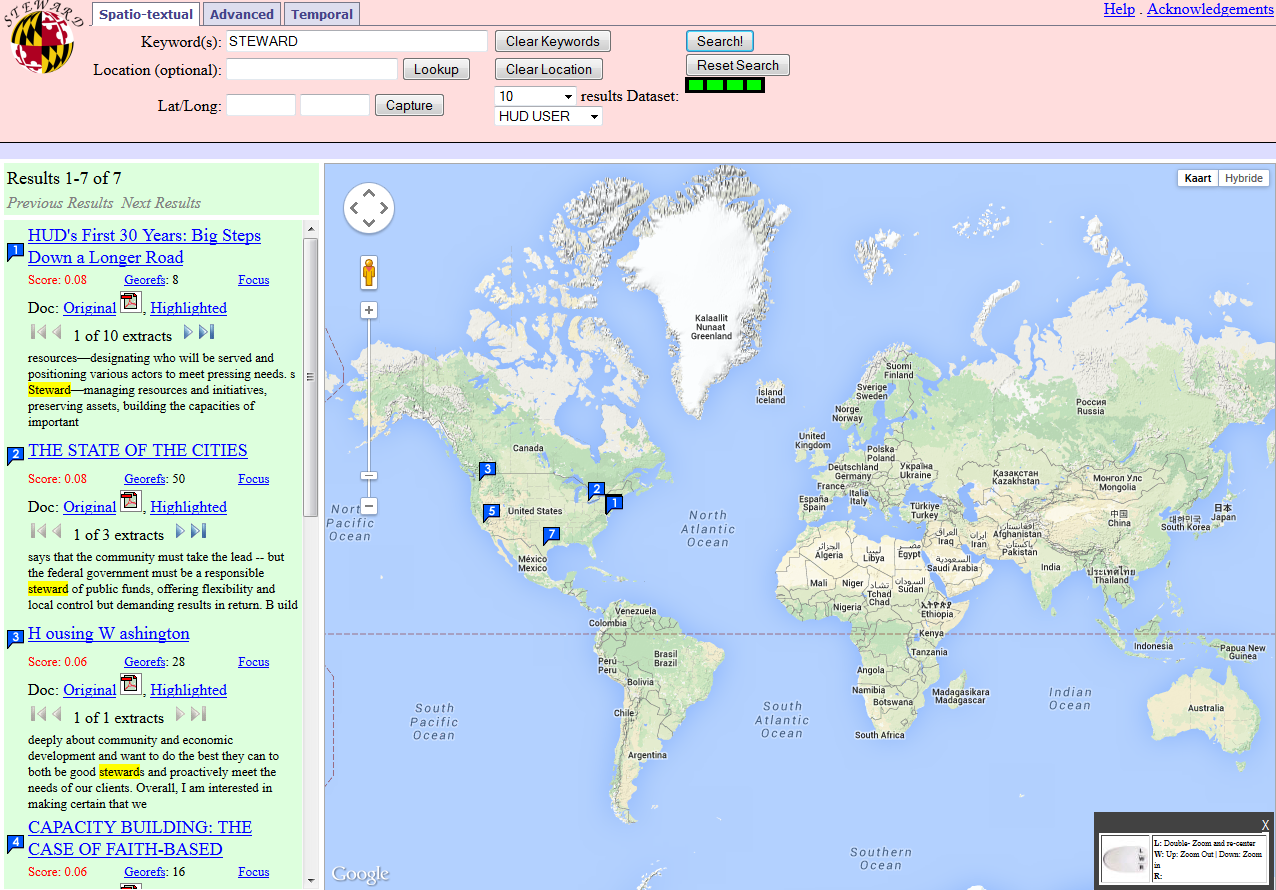
\includegraphics[scale=0.3]{./img/STEWARD.png}
			\caption{STEWARD User Interface}
		\end{figure}
		\\[0.5cm]
		Het STEWARD systeem kan gebruikt worden voor een aantal verschillende toepassingen. Bijvoorbeeld als zoekmachine voor het "hidden web"\footnote{http://en.wikipedia.org/wiki/Deep\_Web}, waar een normale zoekmachine, welke gebruik maakt van een pagerank algoritme\footnote{http://en.wikipedia.org/wiki/PageRank}, niet zal werken door het gebrek aan links naar de documenten. Ook kan er gezocht worden op nieuws, dit gaat nog wel aan de hand van een onderwerp (met eventueel een locatie). De resultaten worden vervolgens op een kaart weer gegeven zodat de gebruiker gemakkelijk kan zien wat de geografische locatie van het artikel is. Daarnaast kan het systeem gebruikt worden als een monitoring systeem voor ziektes, en het verzamelen van touristische, historische en recreationele informatie over een stad of gebied.
	\section{NewsStand: A New View on News \cite{NewsStand2008}}
		Nieuws artikelen bevatten heel veel (implicite) geografische informatie, die niet altijd duidelijk is voor de lezer. Door dit inzichtelijk te maken wordt het begrip van nieuws vergroot. NewsStand doet dit door RSS feeds \footnote{http://en.wikipedia.org/wiki/RSS} in de gaten te houden. Voor elk artikel wordt de geografische inhoud ge"extraheerd door gebruik te maken van een geotagger, de artikelen worden vervolgens geclusterd. Door in te zoomen op de kaart kunnen gebruikers nieuwsberichten vinden, afhankelijk van hoe ver een gebruiker ingezoomd is worden verschillende nieuwsberichten getoond.
		\\[0.5cm]
		In het artikel wordt besproken waarom een dergelijk systeem nuttig is, en hoe dit systeem is opgebouwd.
	\section{Reading News with Maps by Exploiting Spatial Synonyms \cite{RNwMbESS}}
		Dit artikel uit oktober 2014 is het vervolg op \textit{NewsStand: A New View on News} uit november 2008. De architectuur van NewsStand\footnote{http://newsstand.umiacs.umd.edu/web/} wordt ook in dit artikel weer besproken, net als het proces van het geotaggen en de problemen waar hier rekening mee gehouden moeten worden.
		\\[0.5cm]
		In de toekomst willen zij deze tool uitbreiden zodat er naast tekst ook geozcht kan worden op foto's, videos en audio. Ook willen ze andere soorten nieuwsbronnen gaan gebruiken zoals Twitter.
		\begin{figure}[!htb]
			\centering
			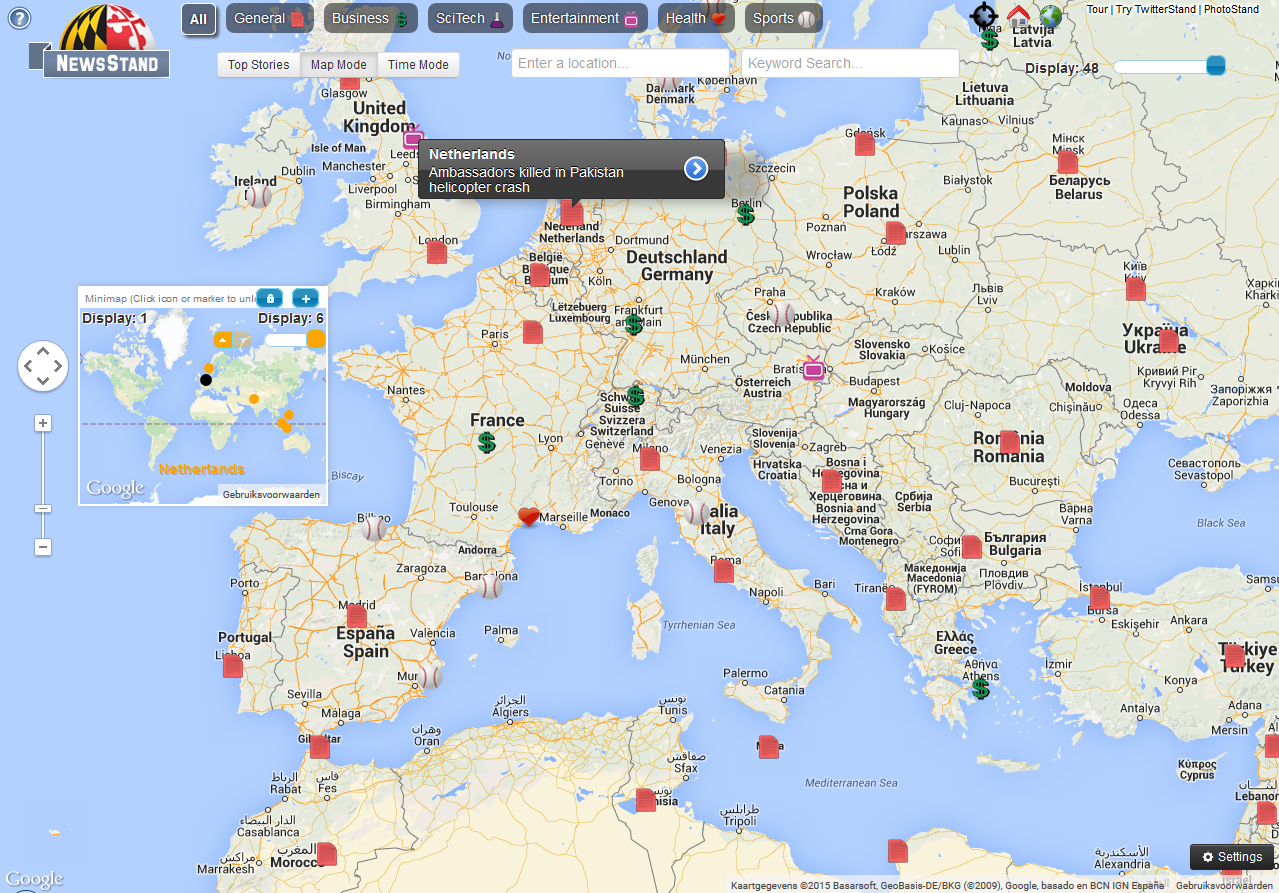
\includegraphics[scale=0.3]{./img/NewsStand.png}
			\caption{NewsStand User Interface}
		\end{figure}
\chapter{Ontwerp}
	In dit hoofdstuk zullen de gemaakte ontwerpkeuzes besproken worden. Ook zullen er twee voorstellen gedaan worden voor de implementaties van een dergelijke applicatie.
	\section{Web applicatie of standalone/desktop applicatie?}
		Een dergelijke applicatie kan ge"implementeerd worden als web applicatie of standalone applicatie. In deze sectie zullen we beide opties bespreken en een keuze tussen deze twee maken.
		\subsection{Web applicatie}
			Een web applicatie is een applicatie die voor gebruikers beschikbaar is via een webserver. Deze server is vaak bereikbaar via het internet maar het is ook mogelijk om dit via intranet te doen. De gebruiker kan via een client programma, zoals een webbrowser, gebruik maken van een dergelijke applicatie.
		\subsection{Standalone/desktop applicatie}
			Een standalone of desktop applicatie is een programma waarbij vooraf bepaald is welek taken uitgevoerd kunnen worden. Vaak zijn dergelijke programma's beschikbaar vanaf een lokale schijf in de computer van een gebruiker en hebben deze programma's in principe geen internet/netwerk nodig om te kunnen functioneren.
		\subsection{Web applicatie vs. standalone/desktop applicatie}
			Hier onder staan voor zowel een web applicatie als een standalone/desktop aplpicatie op een rijtje.\\[0.5cm]
			\textbf{Voordelen web applicatie}
			\begin{itemize}
				\item Snel voor iedereen toegankelijk
				\item Overal beschikbaar (waar internet is)
				\item Geen onderhoud (updates installeren) voor de gebruiker
			\end{itemize}
			\textbf{Voordelen standalone/desktop applicatie}
			\begin{itemize}
				\item Krachtigere software, gebruik maken van hardware features
				\item Veiliger
				\item Lagere kosten voor de gebruiker op de lange termijn
				\item Geen internet verbinding nodig
				\item Sneller
				\item Mogelijkheid om backups van data te maken
			\end{itemize}
			Hier uit blijkt dat een desktop applicatie vooral geschikt is als er bijvoorbeeld grote berekeningen uitgevoerd moeten worden op de computer van de gebruiker. Daarnaast is een desktop applicatie ook sneller als er grote hoeveelheden data in een database opgeslagen moeten worden. Bij een standalone/desktop applicatie kan deze database namelijk op de computer van de gebruiker opgeslagen worden en hoef je alleen naar de schijf te schrijven. Bij een web applicatie zou deze data eerst over een netwerk verstuurd moeten worden om vervoglens alsnog naar een schijf geschreven te worden.\\[0.5cm]
			Voor onze applicatie is het vooral belangrijk dat gebruikers snel en overal bij de applicatie kunnen komen. Verder versturen we geen privacy gevoelige informatie dus de extra veiligheid die en standalone/desktop applicatie biedt heeft geen toegevoegde waarde. Omdat we ook geen grote hoeveelheden data hoeven te versturen en ook geen grote berekeningen op de computer van de gebruiker hoeven uit te voeren is er gekozen om de applicatie te implementeren als web applicatie.
	\section{Server}
		Zoals in de voorgaande sectie beschreven is er gekozen voor een web applicatie. Hiervoor moet een server ge"implementeerd worden, in deze sectie worden de ontwerp keuzes besproken die betrekking hebben op deze web server.
		\section{Python, PHP of Ruby on Rails}
			Drie mogelijke talen om een web applicatie mee te ontwikkelen zijn PHP\footnote{http://php.net/}, Ruby\footnote{https://www.ruby-lang.org/en/} en Python\footnote{https://www.python.org/}, van deze talen is PHP de meest gebruikte. In afbeelding \ref{fig:phpvspython} wordt een vergelijking gemaakt tussen de drie talen. In figuur \ref{fig:phpvspython3} is te zien dat PHP verreweg de meest gebruikte taal is.
			\begin{figure}[!htb]
				\centering
				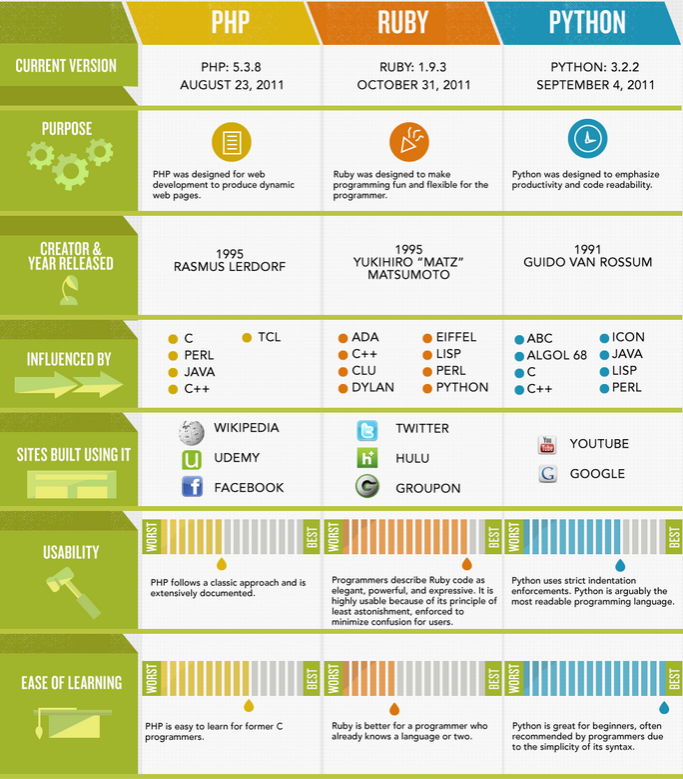
\includegraphics[scale=0.9]{./img/phpvspython.png}
				\caption{Vergelijking PHP, Ruby en Python}
				\label{fig:phpvspython}
			\end{figure} 
			\begin{figure}[!htb]
				\centering
				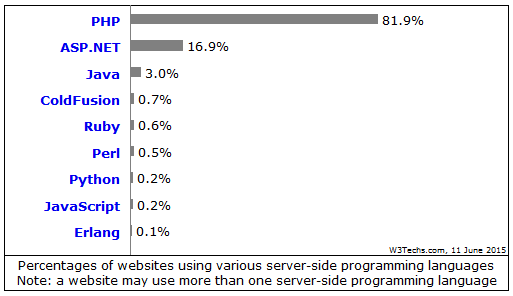
\includegraphics[scale=0.9]{./img/phpvspython3.png}
				\caption{Vergelijking PHP, Ruby en Python}
				\label{fig:phpvspython3}
			\end{figure} 
			\subsection{PHP}
				PHP, \textit{P}HP: \textit{H}ypertext \textit{P}reprocessor, is een scripttaal waarmee dynamische web pagina's ontwikkeld kunnen worden. De taal is in 1994 ontworpen door Rasmus Lerdorf, en ge"inspireerd door Perl\footnote{https://www.perl.org/}. Tegenwoordig is dit de meest gebruikte taal om web applicaties mee te ontwikkelen. 
			\subsection{Ruby}
				Ruby is een programmeertaal waarmee eenvoudig en snel objectge"orienteerd geprogrammeerd kan worden, de taal is in 1995 gepubliceerd door Yukihiro Matsumoto. Sinds 2004 is Ruby on Rails beschikbaar, dit is een open source webapplicatieframework geschreven in Ruby. 
			\subsection{Python}
				Python is een in 1991 verschenen programmeertaal, de taal is door Guido van Rossum ontwikkeld. Het is een van de eenvoudigste talen om te leren en omdat het erg op psuedo code lijkt is het meestal ook goed te lezen en te begrijpen voor mensen die zelf niet kunnen prorgarmmeren.
				\\[0.5cm]
			Voor dit project is gekozen om gebruik te maken van Python, in combinatie met CherryPy en Cheetah. We hebben hier voor gekozen omdat het een stuk sneller is dan PHP qua run time en het aantal regels code nagenoeg gelijk is aan het aantal dat bij PHP nodig zou zijn, zie afbeelding \ref{fig:phpvspython2}. Hierbij is er ook rekening mee gehouden dat met Python ook standalone applicatie gemaakt kunnen worden, wat met PHP (bijna) niet mogelijk is. Op deze manier kan een groot deel van de code direct gebruikt worden als er behoefte is aan een dergelijke applicatie.
			\begin{figure}[!htb]
				\centering
				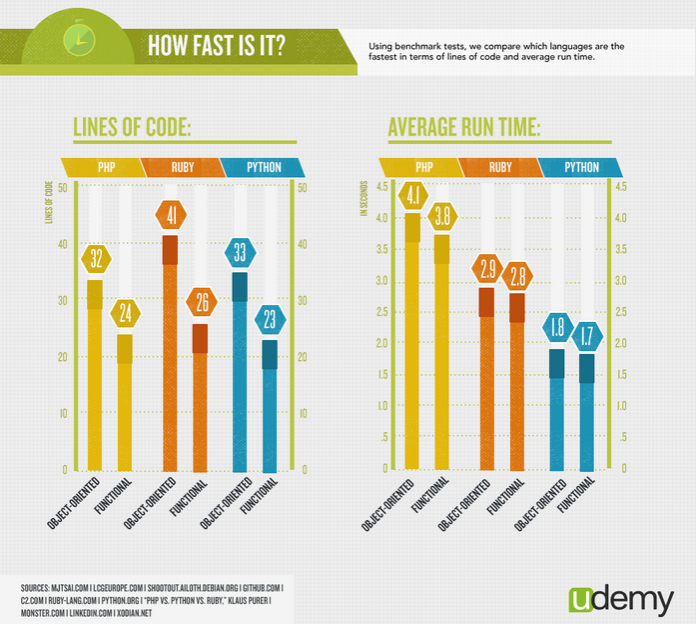
\includegraphics[scale=0.9]{./img/phpvspython2.png}
				\caption{Vergelijking snelheid PHP, Ruby en Python}
				\label{fig:phpvspython2}
			\end{figure}
		\subsection{CherryPy}
			CherryPy\footnote{http://www.cherrypy.org/} is een open-source minimalistisch Python Web Framework, hiermee is het mogelijk om web applicaties te maken op (bijna) de zelfde manier als een object ge"orienteerd Python programma. Het resultaat hiervan is dat er minder code nodig is en het ontwikkelen van een web applicatie minder tijd kost.
			\\[0.5cm]
			Inmiddels bestaat CherryPy al meer dan tien jaar en heeft het bewezen zweer snel en stabiel te zijn. Het wordt gebruikt bij veel websites, van kleine simpele sites tot zeer veel eisende applicaties.
			\\[0.5cm]
			Een voorbeeld van een simpele website met CherryPy is het volgende:
			\begin{verbatim}
			import cherrypy
			
			class HelloWorld(object):
			@cherrypy.expose
			def index(self):
			    return "Hello world!"
			
			if __name__ == '__main__':
			    cherrypy.quickstart(HelloWorld())
			\end{verbatim}
			Deze code start een webserver met de standaar configuratie en print de tekst \"Hello World!\" op de pagina. Het is ook mogelijk om een eigen configuratie voor de server te gebruiken, hierin is \textit{cherry\_conf} een Python dictionary\footnote{https://docs.python.org/2/tutorial/datastructures.html\#dictionaries}. Op deze manier kan er bijvoorbeeld handmatig bepaald worden op welk IP adres de server te vinden is en welke poort, standaard $8080$, er gebruikt wordt. 
			\begin{verbatim}
			cherrypy.quickstart(HelloWorld(), config = cherry_conf)
			\end{verbatim}
			In plaats van een simpele tekst op het scherm willen we graag een complete HTML pagina terug geven, dit doen we door gebruik te maken van Cheetah.
		\subsection{Cheetah}
			Cheetah\footnote{http://www.cheetahtemplate.org/} of Cheetah Template is een template engine die gebruik maakt van Python. Het kan apart gebruikt worden of in combinatie met andere tools en frameworks, zoals bijvoorbeeld CherryPy. Over het algemeen wordt het gebruikt voor server-side scripting en het genereren van dynamische web pagina's. Een simpel voorbeeld is het volgende, deze Cheetah template genereerd een HTML pagina met daarop een tabel waarin voor voor elke client de achternaam en voornaam en een link naar het emailadres een regel wordt gemaakt.
			\begin{verbatim}
			<html>
			    <head>
			        <title>
			            $title
			        </title>
			    </head>
			    <body>
			        <table>
			        #for $client in $clients
			            <tr>
			                <td>
			                    $client.surname, $client.firstname
			                </td>
			                <td>
			                    <a href="mailto:$client.email">$client.email</a>
			                </td>
			            </tr>
			        #end for
			        </table>
			    </body>
			</html>
			\end{verbatim}
			Voor dit project gebruiken we JSON om een template te maken van de User Interface.
		\subsection{JSON}
			JSON\footnote{http://json.org/} staat voor Javascript Object Notation, het is een simpel formaat voor gegevens uitwisseling. Het is gemakkelijk door computers te verwerken en goed leesbaar voor mensen. Na genoeg alle programmeertalen ondersteunen JSON, zo ook Python. Hier onder volgt een voorbeeld van JSON.
			\begin{verbatim}
			[
			    { 
			        "Naam": "JSON",
			        "Type": "Gegevensuitwisselingsformaat",
			        "isProgrammeertaal": false,
			        "Zie ook": [ "XML", "ASN.1" ] 
			    },
			    { 
			        "Naam": "JavaScript",
			        "Type": "Programmeertaal",
			        "isProgrammeertaal": true,
			        "Jaar": 1995 
			    } 
			]
			\end{verbatim}
			Wij gebruiken JSON om de lijst met steden en landen terug te sturen naar de client en de nieuwsberichten worden als JSON object opgevraagd. 
		\subsection{AJAX}
			AJAX\footnote{http://en.wikipedia.org/wiki/Ajax\_(programming)}, \textit{A}synchronous \textit{J}avaScript \textit{A}nd \textit{X}ML, wordt gebruikt bij de ontwikkeling van interactieve web pagina's, waarbij asynchroon gegevens van de server worden opgehaald. Dat wil zeggen dat we niet de hele pagina hoeven te vernieuwen als we bijvoorbeeld een andere afbeelding willen laden. Bij dit project maken we gebruik van AJAX om de co"ordinaten van het middelpunt en de straal van het geselecteerde gebied naar de server te verstruren. Ook het uitvoeren van zoekopdrachten voor nieuwsberichten gaat via AJAX. Hiervoor gebruiken we de standaard functies die voor AJAX in JQuery\footnote{https://jquery.com/} ge"implementeerd zijn.
	\section{Database}
		Voor de database hebben we gekozen voor een SQLite\footnote{http://www.sqlite.org/} database. SQLite is een software pakket wat een SQL database engine implementeerd, maar in tegenstelling tot bijvoorbeeld MySQL is hier geen client/server systeem voor nodig. Bij SQLite wordt de database in \'e\'en bestand op de schijf opgeslagen.
		\\[0.5cm]
		Omdat SQLite standaard geen ondersteuning heeft voor veel wiskundige functies zijn deze toegevoegd via een extentie. Hiervoor wordt het bestand \textit{extension-functions.c} gebruikt. Hierin zijn functies als $\cos$ en $\sin$ ge"implementeerd.
	\section{Geografische informatie}
		\label{sec:geo_info}
		Voor de geografische informatie, de steden met hun lengtegraad en breedtegraad, populatie en landen is gekeken naar de mogelijkheid om dit via Google Maps te doen. Hoewel dit in theorie mogelijk is, is dit in praktijk geen goede optie. We zouden dan alle steden die in Google Maps te vinden zijn eerst moeten downloaden en opslaan in een database voordat we kunnen gaan berekenen of ze in het geselecteerde gebied liggen.
		\\[0.5cm]
		Een andere mogelijkheid waar naar gekeken is, is om gebruik te maken van Wolfram Alpha\footnote{https://www.wolframalpha.com/}, hiermee is het mogelijk om de afstand tussen twee steden op aarde te berkenen. Wel moeten we dan zelf de lengtegraad en breedtegraad van het start en eind punt hebben, we kunnen hiermee dus geen steden zoeken.
		\\[0.5cm]
		GeoNames\footnote{http://www.geonames.org/} is een database waar (vrijwel) alle steden op de wereld in te vinden zijn. De database bevat heel veel informatie waarvan, voor ons, vooral de naam van de stad, de populatie, de lengtegraad en breedtegraad en het land waar de stad in ligt interessant zijn. Voor landen en steden zijn ook alternatieve namen, in andere talen dan Engels, te vinden in de database. Daarnaast zijn ook zee"en, oceanen, meren, bergen etc. op te zoeken. Voor dit project is alleen gekeken naar steden en landen maar voor een toekomstig onderzoek zijn dit interessante opties.
		\\[0.5cm]
		De database is via een API te benaderen of te downloaden als tekst betand. Bij dit project is voor het laatste gekozen om het netwerk verkeer zo beperkt mogelijk te houden en om te zorgen dat de data altijd beschikbaar is. Omdat een tekstbestand niet effici"ent te door zoeken is schrijven we dedata naar onze eigen SQLite database.
		\\[0.5cm]
		Tijdens de ontwikkeling van de applicatie bleek dat voor een deel van de steden, ongeveer $30000$ van de $145000$, geen populatie beschikbaar is. Omdat we bij het algoritme voor de gebiedsrepresentatie kijken wat de grootste stad in een gebied is en dit niet mogelijk is met twee of meer steden waarvan de populatie gelijk is aan $0$ worden deze steden uitgesloten tijdens de selectie. In sectie \ref{sec:citiespop} wordt een voorstel gedaan hoe dit opgelost zou kunnen worden zodat deze steden wel gebruikt kunnen worden. Een ander pboleem wat tijdens de implementatie boven kwam is dat een aantal grote steden, zoals Londen en Parijs, in meerdere delen in de database opgeslagen zijn. Ook dit kan voor problemen zorgen bij het algoritme voor de gebiedsrepresentatie. Een oplossing hiervoor is te vinden in sectie \ref{sec:multcities}.
	\section{Nieuwsbronnen}
		Voor de ontwikkeling van de applicatie is gekeken naar meerdere nieuwsbronnen. Hier zullen we een aantal van deze bronnen bespreken.
		\subsection{Google News}
			Google News is een zoekmachine van Google om nieuws berichten te doorzoeken. De titles, eerste alinea's en afbeeldingen van nieuwsberichten op het internet worden verzameld en kunnen aan de hand van keywords worden doorzocht. Voor deze dienst is een API beschikbaar maar deze wordt sinds 26 mei 2011 niet meer ondersteund. Er kan nog wel gebruik van gemaakt worden, maar de API wordt niet meer bijgewerkt. 
		\subsection{BING News}
			BING News is een vergelijkbare zoekmachine van Microsoft. Ook hier is een API voor beschikbaar, welke nog wel ondersteund wordt. Per maand kunnen hier gratis $5000$ zoekopdrachten mee uitgevoerd worden, mocht er meer nodig zijn dan is dit mogelijk tegen betaling.
		\subsection{Overig}
			Naast Google News en BING News hebben we nog naar een aantal andere optie gekeken.
			\subsubsection{Yahoo News Service}
				Ook deze zoekmachine is te vergelijken met Google News en BING News. Hier voor is ook een API beschikbaar, deze is echter alleen te gebruiken tegen betaling. Voor dit project is dat niet haalbaar maar mogelijk dat dit in de toekomst een interessante optie is.
			\subsubsection{FAROO}
				FAROO\footnote{http://www.faroo.com/hp/api/api.html} is een alternatief voor de hierboven genoemde opties. Het is een gratis zoek API waarbij tot 1 miljoen zoekopdrachten per maand gedaan kunnen worden. 
			\subsubsection{Lokaal nieuws}
				Een hele interessante optie is om lokale nieuws sites en kranten te zoeken bij het geselecteerde gebied. Vooral voor kleinere gebieden, zal dit nuttige resultaten op kunnen leveren. in hoofdstuk \textbf{<todo>} gaan we hier dieper op in.
	\section{Zoeken naar nieuws}
		Het zoeken naar nieuws gaat via de BING API\footnote{http://datamarket.azure.com/dataset/bing/search}. Hiermee is het mogelijk om gratis $5000$ zoekopdrachten per maand uit te voeren, tegen betaling kunnen er meer zoekopdrachten uitgevoerd worden. We zoeken naar nieuws aan de hand van een stad en het land waarin deze stad ligt. Hiervoor is gekozen omdat wanneer we alleen op de naam van een stad zoeken, en deze stad komt in meerdere landen voor, we ook resultaten uit andere landen krijgen die niks met het zoek gebied te maken hebben. 
		\subsection{Client side of server side?}
			Het zoeken naar nieuws kan zowel client side als server side gebeuren.
			Het zoeken van nieuws door de server heeft als voordeel dat het mogelijk is om een cache aan te leggen, van nieuws wat bij een stad hoort. Daarbij komt dat de sleutel van de BING API niet beschikbaar is voor de gebruiker en dus niet misbruikt kan worden. 
			Omdat we voor dit project maar een kleine server beschikbaar hebben is er toch gekozen om dit client side te doen om de server zo min mogelijk te belasten.
	\section{De ideale implementatie}
		In deze sectie beschrijven we een voorstel hoe een dergelijke applicatie eigenlijk zou moeten. Helaas is het vooral door gebrek aan tijd, twaalf weken, niet mogelijk om het op deze manier te doen. 
		\\[0.5cm]
		Zoals eerder gezegd heeft het zoeken naar nieuws door de server een aantal voordelen. Dit zoeken zou dan ook niet meer via bijvoorbeeld BING News gaan, een betere optie is om gebruik te maken van RSS feeds\footnote{http://en.wikipedia.org/wiki/RSS}.
		\subsubsection{RSS feeds}
			RSS staat voor \textit{R}ich \textit{S}ite \textit{S}ummary, maar ook vaak \textit{R}eally \textit{S}imple \textit{S}yndication genoemd, het is een eenvoudige manier om op de hoogte te blijven van bijvoorbeeld het laatste nieuws. Het is gemaakt zodat we niet zelf alle sites hoeven te bezoeken waarvan we op de hoogte willen blijven van de nieuwste berichten. In plaats daarvan kunnen we de RSS feed in de gaten houden, de nieuwste berichten komen hier automatisch op te staan.
			\\[0.5cm]
		Met een achtergrond proces op de server kunnen deze RSS feeds in de gaten gehouden worden en zodra er een nieuw nieuws bericht beschikbaar is wordt deze gedownload. Eenmaal gedownload moet een bericht geanalyseerd worden om te bepalen bij welke stad het bericht hoort. Nieuwsberichten die geanalyseerd zijn worden opgelsagen in een database, met bijvoorbeeld de stad en het land waar het bericht bij hoort, een link naar het bericht en de tijd dat het nieuwsbericht gepubliceerd is. Deze tijd kan gebruikt worden om te bepalen of het nog een actueel bericht is.
		\\[0.5cm]
		Met de hier beschreven methode verstuurt de client alleen nog het middelpunt en de straal van de op de kaart gemaakte selectie. De server doet de rest van het werk, dat wil zeggen het zoeken naar steden die bij het geslecteerde gebied horen, het zoeken naar nieuws dat bij deze steden horen en vervolgens deze lijst met nieuwsberichten terug sturen naar de client. Op deze manier is het ook eenvoudig om nieuwsbronnen toe te voegen, we hoeven alleen de RSS feed van de bron in de gaten te houden.
\chapter{Implementatie}
	Hier onder zullen we de implementatie van de hiervoor gemaakte ontwerpkeuzes beschrijven.
	\begin{figure}[!htb]
		\label{fig:arch}
		\centering
		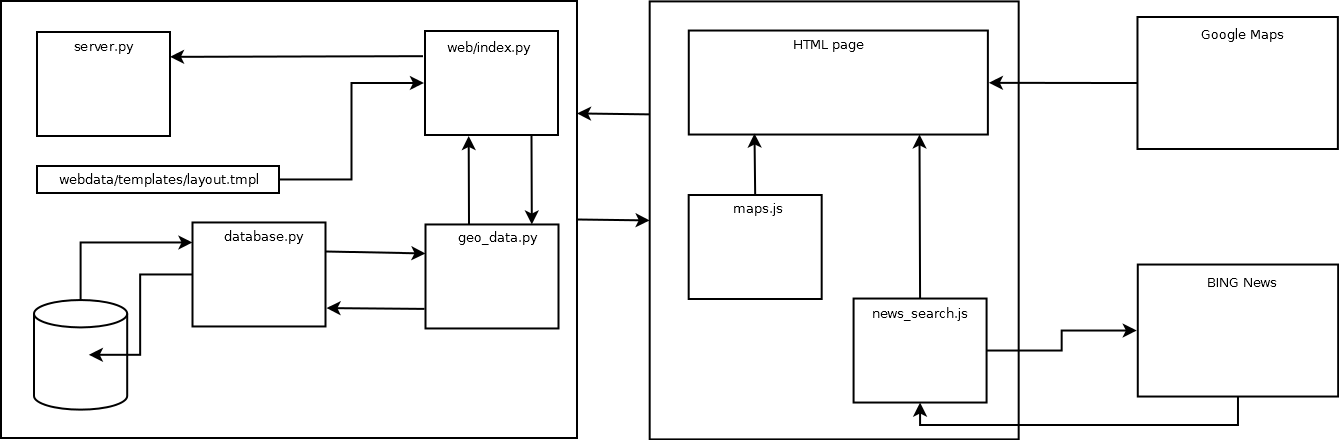
\includegraphics[scale=0.3]{./img/architecture.png}
		\caption{Architectuur}
	\end{figure}
	\section{Server en database}
		\subsection{Server}
		De server is geschreven in Python en maakt gebruik van CherryPy en Cheetah. In principe is de server ge"implementeerd als webserver maar zou ook gebruikt kunnen worden als API\footnote{http://en.wikipedia.org/wiki/Application\_programming\_interface} voor een andere applicatie.
		
		\subsubsection{Webserver}
		Op de webserver draait \'e\'en pagina, \textit{web/index.py}, de template met daarin alle HTML voor deze pagina is te vinden in \textit{webdata/templats/layout.tmpl}.
		\\[0.5cm]
		Wanneer \textit{web/index.py} een HTTP GET request\footnote{http://en.wikipedia.org/wiki/Hypertext\_Transfer\_Protocol\#Request\_methods} krijgt wordt de HTML uit deze template terug gestuurd naar de gebruiker.
		\\[0.5cm]
		Zodra een gebruiker een gebied op de kaart selecteerd wordt er een HTTP POST request door de client naar de server gestuurd. De door de client opgestuurde data, de lengtegraad en breedtegraad van het middelpunt en straal van het gebied, wordt gecontrolleerd en de steden die bij dit gebied horen worden opgezocht. Deze steden worden in een JSON object terug gestuurd naar de client.
		\subsubsection{API}
		Om de server te gebruiken als API voor een andere applicatie maken we alleen gebruik van de HTTP POST request, hierin sturen we de lengtegraad en breedtegraad van het middelpunt en de straal van het gebied. Vervolgens krijgen we een JSON object terug met de steden die dit gebied representeren welke we verder kunnen verwerken voor onze applicatie.
		\textit{TODO: voorbeeld}
		\subsection{Database}
			Zoals uitgelegd in sectie \ref{sec:db} maken we gebruik van een SQLite database, Python heeft hier ondersteuning voor via de \textit{sqlite3}\footnote{https://docs.python.org/2/library/sqlite3.html} module.\\[0.5cm]
			De database, afbeelding\ref{fig:db} bevat twee tabellen, \textit{cities} en \textit{countries}. De \textit{cities} tabel bevat alle steden, elke stad in de tabel heeft een uniek ID, een naam, een aantal inwoners, een code voor het land waarin deze stad ligt en de co\"ordinaten, breedtegraad en lengtegraad, van de stad. De landcode verwijst naar de tabel \textit{countries}, hiermee kan de naam van het land waarin de stad ligt opgezocht worden. \\[0.5cm]
			De tweede tabel in de database is de \textit{countries} tabel,  met velden voor de naam en de code van het land.
			\begin{figure}[!htb]
				\label{fig:db}
				\centering
				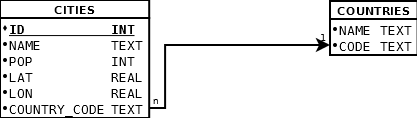
\includegraphics[scale=0.6]{./img/database.png}
				\caption{Database}
			\end{figure}
			\subsubsection{database.py}
			Bij een SQL query is een groot deel van de query vast, bij bijvoorbeeld een SELECT query veranderen alleen de naam van de tabel en de velden die we willen selecteren.
\begin{verbatim}
SELECT x, y, z FROM table;
\end{verbatim}
			Om niet elke keer een hele query te moeten maken staan er in dit bestand functies waarbij we aan kunnen geven welke velden van welke tabel we willen selecteren, de functie maakt de SQL query en voert deze ook direct uit. Er zijn functies voor het selecteren, toevoegen, updaten en verwijderen van entries in de database. Daarnaast zijn er ook functies voor het maken en verwijderen van tabellen.
		\subsection{geo\_data.py}
		In dit Python bestand staan functies voor het downloaden van de geografische informatie van \textit{geonames.org}. Deze informatie is beschikbaar in een tekst bestand, omdat dit niet effici"ent is als er gekeken moet worden welke steden er in een gebied liggen is er een functie om deze data naar de database te schrijven. In principe wordt dit alleen de eerste keer gedaan, maar mocht het nodig zijn kan de database opnieuw opgebouwd worden.\\[0.5cm]
		Behalve de functies om de database te downloaden en op te bouwen zijn er ook functies om de steden te zoeken en een algoritme om te bepalen welke steden het gebied representeren is hier ge"implementeerd.
	\section{Welke steden liggen in het geselecteerde gebied?}
		Een door de gebruiker op de kaart geselecteerd gebied wordt weergegeven door de co\"ordinaten van het middelpunt (breedtegraad\footnote{http://en.wikipedia.org/wiki/Latitude} en lengtegraad\footnote{http://en.wikipedia.org/wiki/Longitude}) en de straal van de cirkel (het gebied) in kilometers.
		\\[0.5cm]
		Om te berekenen welke steden binnen dit gebied ligen moet de afstand van het middelpunt tot een stad berekend worden. Is deze afstand kleiner dan of gelijk aan de straal van het geselecteerde gebied, dan ligt de stad in het gebied.
		\\[0.5cm]
		Voor het berekenen van de afstand tussen twee punte $P_1(lat_1, lon_1)$ en $P_2(lat_2, lon_2)$ op een bol, zoals de aarde,  kan geen gebruik gemaakt worden van de stelling van Pythagoras\footnote{http://en.wikipedia.org/wiki/Pythagorean\_theorem} omdat deze stelling uit gaat van een plat vlak. Om de afstand tussen twee punten op een bol te berekenen kan gebruik gemaakt worden van bijvoorbeeld de \textit{spherical law of cosines}\footnote{http://en.wikipedia.org/wiki/Spherical\_law\_of\_cosines} of de \textit{haversine formule}\footnote{http://en.wikipedia.org/wiki/Haversine\_formula}. De \textit{haversine formule} is vooral voor kleine afstanden nauwkeuriger, met deze formule kunnen afstanden tot ongeveer 'e'en meter nauwkeurig berekend worden. Bij de \textit{spherical laq of cosines} is de maximale fout een paar meter. Om deze reden wordt de \textit{haversine formule} meer gebruikt bij navigatie, voor dit project is een fout van een paar meter echter niet belangrijk. Er is daarom gekozen voor de \textit{spherical law of cosines}.
		\\[0.5cm]
		$distance = \arccos(\sin(lat_1) \cdot \sin(lat_2) + \cos(lat_1) \cdot \cos(lat_2) \cdot(lon_1 - lon_2)) \cdot R$
		\\[0.5cm]
		Hierin zijn $(lat_1, lon_1)$ de co"ordinaten van het startpunt, in dit geval het middelpunt van het geselecteerde gebied, en $(lat_2, lon_2)$ de co"ordinaten van het tweede punt waarvoor we de afstand tot het start punt willen berekenen. Deze co"ordinaten worden door de client in graden door gestuurd en moeten eerst omgezet worden naar radialen om in deze formule gebruikt te kunnen worden. $R$ is de straal van de bol waarop beide punten liggen, in dit geval de aarde $ 	\Rightarrow R = 6371km$.
		\\[0.5cm]
		Met deze formule zou meteen een \textit{SQL\footnote{http://en.wikipedia.org/wiki/SQL} query} geconstrueerd kunnen worden.
\begin{verbatim}
SELECT
    cities.NAME, cities.LAT, cities.LON, cities.POP
FROM 
    cities 
WHERE 
    acos(sin(lat) * sin(cities.lat) + cos(lat) * cos(cities.lat) * cos(lon - cities.lon)) * 
    6371 <= radius;
\end{verbatim}
		Deze query geeft als resultaat een lijst met steden die binnen het door de gebruiker geselecteerde gebied liggen. Voor elke stad wordt de naam, populatie, breedtegraad en lengtegraad terug gegeven.
		\\[0.5cm]
		Nadeel van deze query is echter dat voor alle steden in de database berekend moet worden of de afstand tot het middelpunt van het geselecteerde gebied kleiner dan of gelijk is aan de straal van het gebied. Dit kost veel tijd, om dit te versnellen selecteren we alleen kandidaat steden waar we vervolgens de berekening op uit gaan voeren. Door de minimale en maximale breedtegraad en lengtegraad te berekenen kunnen we al een heleboel steden uitsluiten die sowieso buiten het geselecteerde gebied liggen.
		\subsubsection{Berekenen minimale en maximale breedtegraad}
		Als je van een punt $A$ naar een punt $B$ op een cirkel gaa tkun je de hoek, $r$, tussen deze twee punten berekenen. Lengtecirkels (meridianen)\footnote{http://en.wikipedia.org/wiki/Meridian\_(geography)} zijn dergelijke cirkles op aarde met een straal van $R = 6371km$. Je kan dus over een meridiaan verplaatsen, dat wil zeggen de lengtegraad blijft constant, en simpelweg $r$ aftrekken/optellen bij de breedtegraad van het middelpunte van het geselecteerde gebied om de minimale en maximale breedtegraad te krijgen.
		\\[0.5cm]
		$lat_{min} = lat - r$ \\
		$lat_{max} = lat + r$
		\\[0.5cm]
		$r$ hangt af van de afstand tussen de twee punten en de straal $R$ van de aarde. De afstand tussen de twee punten stellen we gelijk aan de maximale afstand dat een stad nog in het geselecteerde gebied ligt, dat is de straal van het gebied.
		\\[0.5cm]
		$r = \frac{max. distance}{R} = \frac{radius}{R}$
		\subsubsection{Berekenen minimale en maximale lengtegraad (methode 1)}
		Een door veel applicatie gebruikte benadering om de minimale en maximale lengtegraad te berekenen is een vasta breedtegraad kiezen en de lengtegraad aanpassen. dat betekent dat er over een breedtecirkel\footnote{http://en.wikipedia.org/wiki/Circle\_of\_latitude} bewogen wordt. In deze sectie zullen we aan de hand van een voorbeeld laten zien dat dit geen nauwkeurige resultaten geeft.
		\\[0.5cm]
		Als we over een breedtecirkel bewegen, bewegen we over een zogenaamde kleine cirkel\footnote{http://en.wikipedia.org/wiki/Circle\_of\_a\_sphere}. Een breedtecirkel op breedtegraad $lat = 1.3963$ heeft een straal $R_{S} = R \cdot \cos(lat) = 6371 \cdot \cos(1.3963) = 1106km$. Een afstand van $1000km$ op deze breedtecirkel komt nu overeen met een hoek $r_{S} = \frac{d}{R_{S}} = \frac{1000}{1106} = 0.9039$ tussen twee punten op deze cirkel. Bij een lengtegraad van $-0.6981$ van het beginpunt komen de minimale en maximale lengtegraad nu op
		\\[0.5cm]
		$lon_{min} = -0.6981 - 0.9039 = -1.6020$\\
		$lon_{max} = -0.6981 + 0.9039 = 0.2058$\\[0.5cm]
		Dit is echter \textbf{niet} de minimale en maximale lengtegraad die we kunnen bereiken door $1000km$ in een willekeurige richting te bewegen vanaf het beginpunt $M = (1.3969, -0.6981)$. Dat komt omdat we ons verplaatsen over een kleine cirkel, afstanden over een kleine cirkel zijn groter dan over een grote cirkel\footnote{http://en.wikipedia.org/wiki/Great\_circle}. Hoewel we dus $1000km$ afgelegd hebben op een kleine cirkel om van $M = (1.3969, -0.6981)$ naar $P_{S} = (1.3969, -1.6020)$ kunnen we ``afsnijden'' op een grote cirkel. Deze afstand is\\[0.5cm]		
		$dist = \arccos(\sin(lat_1) \cdot \sin(lat_2) + \cos(lat_1) \cdot \cos(lat_2) \cdot \cos(lon_1 - lon_2)) \cdot R$\\
		$= \arccos(\sin(1.3963) \cdot \sin(1.3963) + \cos(1.3963) \cdot \cos(1.3963) \cdot \cos(-0.6981 - (-1.6020))) \cdot 6371$\\
		$= 967km$\\[0.5cm]
		We kunnen dus nog $33km$ verder verplaatsen en zitten dan nog steeds binnen het geselecteerde gebied, dat wil zeggen dat we een kleinere en grotere minimale en maximale lengtegraad kunnen bereiken.\\[0.5cm]
		Als we dus gebruik maken van $lon \pm \frac{d}{\cos(lat)}$ als grenzen voor de lengtegraad, sluiten we een aantal plaatsen uit die in werkelijkheid wel in het gebied liggen. Een punt $P = (1.4618, -1.6021)$ ligt buiten de berekende grenzen voor een gebied met middelpunt $M = (1.3969, -0.6981)$ en straal $d = 1000km$  terwijl de afstand van $M$ maar $872km$ is, een fout van meer dan $12\%$.
		\subsubsection{Berekenen minimale en maximale lengtegraad (methode 2)}
		De methode omschreven in de vorige sectie om de minimale en maximale lengtegraad te berekenen werkt dus niet goed. Dit is te zien in figuur \ref{fig:tangentpoints}, de punten op de cirkel met de minimale en maximale lengtegraad $T_1$ en $T_2$ liggen niet op de zelfde breedtecirkel\footnote{http://en.wikipedia.org/wiki/Circle\_of\_latitude} als $M$, het middelpunt van het geselecteerde gebied maar dichter bij de pool.
		\begin{figure}[!htb]
			\centering
			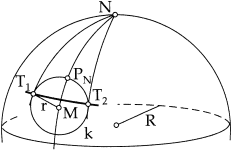
\includegraphics[scale=1.0]{./img/TangentPoints.png}
			\caption{Tangent meridians to the query circle}
			\label{fig:tangentpoints}
		\end{figure}
		\newpage
		In plaats daar van moeten de volgende formules gebruikt worden
		\\[0.5cm]
		$lat_T = \arcsin(\frac{\sin(lat)}{\cos(r)})$\\
		$\Delta lon = \arccos(\frac{\cos(r) - \sin(lat_T) \cdot \sin(lat)}{\cos(lat_T) \cdot \cos(lat)})$ \\
		$= \arcsin(\frac{\sin(r)}{cos(lat)})$
		\\[0.5cm]
		$lon_{min} = lon_{T_1} = lon - \Delta lon$\\
		$lon_{max} = lon_{T_2} = lon + \Delta lon$
		\subsubsection{SQL query}
		Aan dde hand van de hierboven berekende minimale en maximale breedtegraad en lengtegraad kunnen we nu een SQL query maken die de berekening, de spherical law of cosines, alleen hoeft uit te voeren op een veel kleiner aantal kandidaat plaatsen.
\begin{verbatim}
SELECT
    cities.NAME, cities.LAT, cities.LON, cities.POP
FROM 
    cities 
WHERE 
        (cities.LAT >= lat_min AND cities.LAT <= lat_max) 
    AND 
        (cities.LON >= lon_min AND cities.LON <= lon_max) 
GROUP BY
    cities.NAME
HAVING
    acos(sin(lat) * sin(cities.LAT) + cos(lat) * cos(cities.LAT) * 
         cos(cities.LON - (lon))) <= radius;
\end{verbatim}
Deze query selecteerd de naam, breedtegraad, lengtegraad en populatie voor elke stad die binnen het geselecteerde gebied valt. Eerst worden alle steden geselecteerd waarvoor de breedtegraad en de lengtegraad binnen de minimale en maximale waardes vallen. Vervolgens wordt voor elk van deze kandidaat plaatsen uitgerekend of deze ook echt binnen het geselecteerde gebied liggen. De query is vervolgens aangepast om ook de landen waarin de steden liggen te selecteren. Dit is nodig omdat sommige steden in meerdere landen voorkomen. Doe je dit niet kan het voorkomen dat je nieuws uit een heel ander wereld deel krijgt dan het gebied wat de gebruiker geselecteerd heeft.
\begin{verbatim}
SELECT
    cities.NAME, cities.LAT, cities.LON, cities.POP, countries.NAME
FROM 
    cities, countries 
WHERE
        cities.COUNTRY_CODE = countries.CODE 
    AND
        (cities.LAT >= lat_min AND cities.LAT <= lat_max) 
    AND 
        (cities.LON >= lon_min AND cities.LON <= lon_max) 
GROUP BY
    cities.NAME
HAVING
    acos(sin(lat) * sin(cities.LAT) + cos(lat) * cos(cities.LAT) * 
         cos(cities.LON - (lon))) <= radius;
\end{verbatim}
% CONTROLEREN!
Omdat een deel van de steden in de database een populatie van $0$ heeft (ongeveer $30000$ van de $ 140000$ steden), en het algoritme voor de gebiedsrepresentatie de grootste stad in een gebied moet vinden selecteren we alleen de steden waarvan de populatie \textbf{niet} $0$ is.
\begin{verbatim}
SELECT
    cities.NAME, cities.LAT, cities.LON, cities.POP, countries.NAME
FROM 
    cities, countries 
WHERE
        cities.COUNTRY_CODE = countries.CODE 
    AND
        (cities.LAT >= lat_min AND cities.LAT <= lat_max) 
    AND 
        (cities.LON >= lon_min AND cities.LON <= lon_max)
    AND
        cities.pop != 0
GROUP BY
    cities.NAME
HAVING
    acos(sin(lat) * sin(cities.LAT) + cos(lat) * cos(cities.LAT) * 
         cos(cities.LON - (lon))) <= radius;
\end{verbatim}
	\section{Gebieds representatie}
		Bij het geselecteerde gebied worden vaak honderd of meer, en bij een groot gebied duizenden, steden gevonden die in dit gebied liggen. Om voor elke stad naar nieuws te zoeken levert evenveel zoekopdrachten als steden op. Dit gaat erg veel tijd in beslag nemen, ongeveer $300ms$ per zoekopdracht, en levert te veel nieuws op. Een dergelijke hoeveelheid nieuws, in de orde van duidezenden artikelen, is voor de gebruker niet te verwerken en draagt niet bij aan een beter begrip van het nieuws en wat er in het gebied gaande is.
		\\[0.5cm]
		Een gebied moet dus door een kleiner aantal steden gerepresenteerd worden zodat het aantal zoekopdrachten beperkt blijft en de gebruiker de hoeveelheid nieuws goed kan verwerken. Hiervoor zijn verschillende optie die hieronder besproken zullen worden.
		
		\subsubsection{Aantal steden om een gebied te representeren}
			Het aantal steden om een gebied te representeren is bepaald aan de hand van een gebruikersonderzoek. De opzet en resultaten van dit onderzoek worden bepsroken in sectie \ref{sec:numcities}.
		\subsection{Algoritme 1}
			Dit algoritme reduceerd een lijst steden tot een maximum aantal zodat een gebied goed gerepresenteerd wordt. Dit gaat op de volgende manier:
			\begin{algorithm}
				\caption{Algortime 1 voor gebiedsrepresentatie}
				\mbox{Split():}\\[0.5cm]
				\KwIn{list of cities}
				\KwResult{Reduced list of cities representing the area}
				\mbox{}\\
				\While{number of result $<$ number of cities to represent the area}{
						find biggest city;\\
						add to result;\\
						\mbox{}\\
						\ForEach{city}{
							calculate bearing;\\
							add to corresponding sublist (nw/ne/se/sw);
							}
							\mbox{}\\
						\ForEach{sublist (nw/ne/se/sw)}{
							\eIf{number of cities $<= 5$}{
								find biggest city;\\
								add to result;
								}{
								Split(sublist);\\
								add to result;
								}
							}
					}
			\end{algorithm}\\[0.5cm]
			Dit recursieve algoritme heeft als input een lijst met steden, dit zijn in eerste instantie alle steden die in het door de gebruiker op de kaart geselecteerde gebied liggen. De grootste stad in dit gebied wordt gezocht ena an het eind resultaat toegevoegd. Vervolgens wordt het gebied in vier delen opgedeeld: Noord-Oost, Zuid-Oost, Zuid-West en Noord-West, zie figuur \ref{fig:bearing}. Om deze opdeling te maken wordt voor elke stad de richting, ten opzichte van de gootste stad, berekend (algoritme \ref{alg:bearing}) en aan het juiste deel gebied toegevoegd.
			\begin{figure}[!htb]
				\centering
				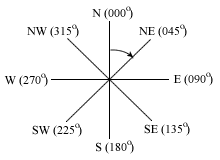
\includegraphics[scale=1.0]{./img/bearings.png}
				\caption{Deelgebieden en hun richting}
				\label{fig:bearing}
			\end{figure}
			\begin{algorithm}
				\caption{Berekenen van de richting}
				\label{alg:bearing}
				\mbox{GetBearing():}\\[0.5cm]
				\KwIn{$(lat_1, lon_1)$, $(lat_2, lon_2)$}
				\KwOut{Bearing in degrees}
				\mbox{}\\
				convert $(lat_1, lon_1)$, $(lat_2, lon_2)$ to radians;\\
				\mbox{}\\
				$\Delta lon = lon_2 - lon_1;$\\
				\mbox{}\\
				$x = \sin(\Delta lon) \cdot \cos(lat_2);$\\
				$y = \cos(lat_1) \cdot \sin(lat_2) - (\sin(lat_1) \cdot \cos(lat_2) \cdot \cos(\Delta lon));$\\
				\mbox{}\\
				$bearing = \arctan(\frac{x}{y});$\\
				\mbox{}\\
				convert bearing to degrees;\\
				\mbox{}\\
				$bearing = \frac{bearing + 360.0}{360.0};$\\
			\end{algorithm}
			Als het aantal steden in een deel gebied kleiner dan of gelijk is aan $5$ wordt de grootste stad in het deelgebied gezocht en aan het eind resultaat toegevoegd. Is het aantal steden echter groter dan wordt het hier boven beschreven proces herhaald voor het deelgebied. \\[0.5cm]
			Aan het einde geeft dit algoritme een lijst van steden die het gebied representeren. Als deze lijst nog steeds meer steden bevat dan het maximale aantal steden om een gebied te representeren wordt dit proces herhaald.
		\subsection{Algoritme 2}
			Een andere mogelijkehid om een aantal steden die een gebied vertegenwoordigen te selecteren is weer de gootste stad kiezen maar nu het gebied in twee delen splitsen in plaats van vier zoals bij het hier boven beschreven algortime.
			\begin{algorithm}
				\caption{Algoritme 2 voor gebiedsrepresentatie}
				\mbox{Split():}\\[0.5cm]
				\KwIn{list of cities}
				\KwResult{Reduced list of cities representing the area}
				\mbox{}\\
				t: list of list of cities;\\
				\mbox{}\\
				\While{number of result $<$ number of cities to represent the area}{
					\ForEach{list in t}{
						\eIf{direction = n/s}{
							biggest, north, south = split\_north(list);\\append biggest to results;\\
							append north, south to t;\\
							remove list from t;\\
							\If{last list in t}{
								set direction to e/w;	
							}	
						}{
						biggest, east, west = split\_east(list);\\append biggest to results;\\
						append north, south to t;\\
						remove list from t;\\
						\If{last list in t}{
							set direction to n/s;	
						}
						}	
					}
				}
			\end{algorithm}\\[0.5cm]
			Het algoritme kiest de grootste stad in het gebied, vevolgens wordt er gekeken welke steden ten noorde liggen en welke steden ten zuide. Voor elk van deze twee deel gebieden wordt weer de grootste stad gezocht, en daarna worden deze deel gebieden opnieuw gesplitst maar nu in oost en west.\\[0.5cm]
			Voor elk deel gebied wordt dus telkens de grootste staad gezocht en deze wordt aan het eind resultaat toegevoegd. het splitsen van een deelgebied gaat om en om: eerst wordt het gebied in noord en zuid gesplitst, dan wordt elk deel gebied in oost en west gesplitst. Nu hebben we vier deelgebieden die allen weer in noord en zuid worden verdeeld etc.
		\subsection{Andere opties}
			Naast deze twee algoritmes zijn er nog enkele andere mogelijkheden om steden te kiezen om een gebied te representeren. Deze werken echter minder goed dan de hier boven beschreven algoritmes.
			\subsubsection{Grootste steden}
				Een mogelijkheid is om alleen de grootste steden in een gebied te selecteren. Voordeel is dat dit een snel en eenvoudig proces is, nadeel is echter dat de verdeling van de grote steden over het gebied (vaak) niet uniform is met als gevolg dat de geselecteerde steden geen goede representatie van het gebied geven.
				%IMAGE
				Een ander probleem bij het selecteren van alleen de grootste steden is dat grote steden, zoals bijvoorbeeld Londen, in meerdere delen in de database staan. Als je nu de grootste steden kiest worden vaak alle drie de delen gekozen met als gevolg dat er clusters ontstaan en er minder steden in de rest van het gebied gekozen kunnen worden.
			\subsubsection{Hoofdsteden}
				In het geval van een selectie van meerdere landen is het een mogelijkheid om alleen de hoofdsteden te gebruiken voor de representatie eventueel aangevuld met de grootste steden in het gebied om voldoende steden te krijgen. Dit is eigenlijk alleen een goede optie als er precies even veel landen als benodigde steden in het gebied liggen. Liggen er minder landen in het gebied, en wordt er aangevuld met de grootste steden, loop je hoogst waarschijnlijk tegen het zelfde probleem aan als wanneer je alleen maar voor de grootste steden kiest. Daarbij komt dat het resultaat vaak nagenoeg gelijk zal zijn omdat hoofdsteden vaak bij de grotere steden horen. 
			\subsubsection{Willekeurig}
				Uit de lijst met steden die in het gebied liggen kunnen willekeurig een aantal steden gekozen worden welke dit gebied representeren. Omdat het hier mogelijk is dat alleen (of grotendeels) kleine/de kleinste steden gekozen worden is dit een minder geschikte mogelijkheid.  Ook is het, net als bij boven genomende methodes, mogelijk dat de gekozen steden niet verspreid liggen maar zich concentreren in een klein deel van het gebied. Ander groot probleem is dat elke keer dat de gebruiker een gebied selecteert een andere lijst aan steden terug gegeven wordt, hierdoor zullen er elke keer andere nieuws artikelen gezocht worden. Het wordt hierdoor moeilijker (onmogelijk) om een artikel opnieuw op te zoeken met de tool.
		\section{User Interface}
		De User Interface is te zien in afbeelding \ref{fig:UI}. Aan de linker kant is een kaart te zien waar de gebruiker met de muis een gebied, in de vorm van een cirkel, kan selecteren. Het selecteren van een gebied gaat als volgt:
		\begin{itemize}
			\item Linker muisklik op de kaart waar het middelpunt van het gebied komt
			\item{Ingedrukt houden en slepen, er is nu een groene cirkel te zien}
			\item{Los laten als het gebied de gewenste grootte heeft}
		\end{itemize}
		Aan de rechter kant is een grijs veld waarin een lijst met links naar nieuws artikelen voor het geselecteerde gebied weer gegeven wordt.
\chapter{Experimenten}
	Om te weten of de ontwikkelde applicatie echt een toegevoegde waarde is moeten er een gebruikers onderzoek uitgevoerd worden. Daarnaast is er een onderzoek nodig om een te bepalen hoeveel steden er nodig zijn om een gebied te representeren, en om een keuze te maken uit de twee voorgestelde algoritmes om deze steden te kiezen.
	\section{Gebiedsrepresentatie}
	\label{sec:numcities}
		Dit onderzoek is gedaan om te bepalen hoeveel steden er nodig zijn om een gebied goed te representeren. Ook wordt er gekeken welke van de twee voorgestelde algoritmes het beste is om de steden te selecteren die het gebied gaan representeren.
		\subsection{Opzet}
			Voor dit experiment is een enqu\^ete gemaakt waarin de gebruiker een afbeelding van een geselecteerd gebied te zien krijgt. Een voorbeeld hiervan wordt gegeven in afbeelding \ref{fig:area_rep}.
			\begin{figure}[!htb]
				\centering
				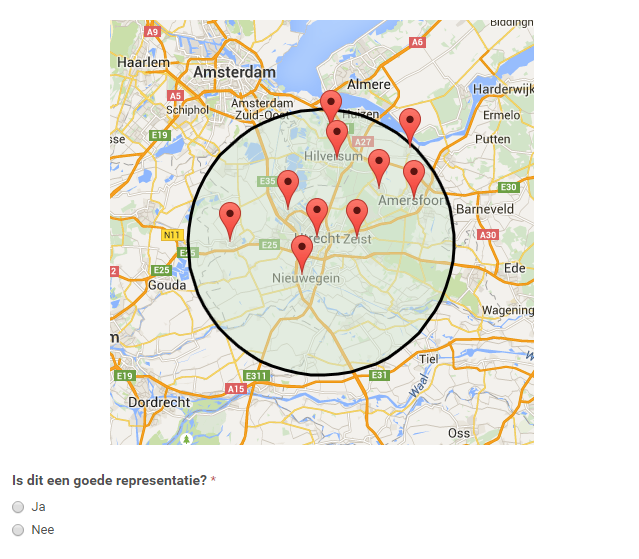
\includegraphics[scale=0.8]{./img/area_rep.png}
				\caption{Voorbeeld vraag gebiedsrepresentatie}
				\label{fig:area_rep}
			\end{figure}
			Bij elke afbeelding krijgt de gebruiker de vraag of dit een goede representatie is van het geselecteerde gebied. Dit is een meerkeuze vraag met als mogelijke antwoorden \textit{ja} en \textit{nee}. Wanneer de gebruiker \textit{nee} kiest krijgt hij of zij een afbeelding van het zelfde gebied te zien maar met meer steden. Er zijn afbeeldingen met tien, vijftien en twintig steden. Zodra er ja gekozen wordt krijgt de gebruiker een vervolg vraag om te bepalen welke van de twee voorgestelde algoritmes beter is. Hiervoor krijgt hij of zij twee afbeeldingen van het zelfde gebied te zien, met het door hem of haar gekozen aantal steden. Een van de afbeeldingen is met algoritme 1 gemaakt terwijl de andere algoritme 2 gebruikt. De vraag is nu welke van de twee representaties beter is, met als mogelijke antwoorden optie 1 of optie 2. Afbeelding \ref{fig:algo} is hier een voorbeeld van. In totaal zijn er voor vier gebebied vragen, dit zijn gebieden met een straal van $25km$, $100km$, $500km$ en $1000km$.
			\\[0.5cm]
			Deze enqu\^ete is in met Google Docs\footnote{http://docs.google.com/} gemaakt en de resultaten worden in een \textit{.xls} bestand opgeslagen.
			\begin{figure}[!htb]
				\centering
				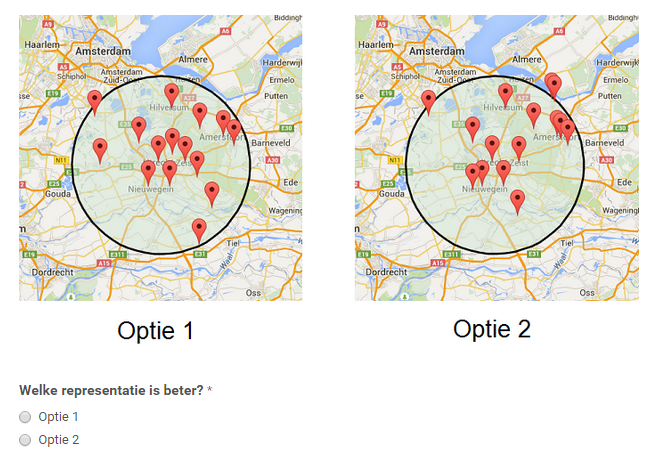
\includegraphics[scale=0.8]{./img/algo.png}
				\caption{Voorbeeld vraag gebiedsrepresentatie}
				\label{fig:algo}
			\end{figure}	
		\newpage		
		\subsection{Resultaten}
			De resultaten zoals deze in het \textit{.xls} bestand opgeslagen zijn zijn te vinden in bijlage \ref{app:results_rep}. Hier onder worden de resultaten per gebied besproken. De enqu\^ete is door twintig mensen ingevuld met een leeftijd van 15 tot en met 80 jaar. Er zitten ongeveer evenveel mannen als vrouwen in deze groep met allemaal een verschillend opleidings niveau. Dit is gedaan om een zo goed mogelijk beeld te krijgen van de hoeveelheid steden die nodig is en wat het beste algoritme is.
			\subsubsection{Gebied 1 - straal 25km}
				In tabel \ref{tab:res25} zijn de resultaten te zien voor een gebied met een straal van $25km$. Aan de hand van deze resultaten kunnen we het gemiddelde aantal steden berekenen dat nodig is om dit gebied te representeren: $\frac{10 * 10 + 9 * 15 + 2 * 20}{21} \approx 13.09$ steden. Verder is te zien dat $\frac{19}{21}  * 100\%\approx 90.48\%$ van de respondenten de representatie gegeven door algoritme 1 beter vindt, $\frac{2}{21} * 100\% \approx 9.52\%$ kiest voor algoritme 2.
				\begin{table}[!htb]
					\centering
					\begin{tabular}{| c | c | c | c | c |}
						\hline	
						\textbf{Kandidaat} & \textbf{10 steden} & \textbf{15 steden} & \textbf{20 steden} & \textbf{Algoritme} \\ \hline
						1 & \ding{56} & \ding{52} &  & 1 \\ \hline
						2 & \ding{56} & \ding{52} &  & 1 \\ \hline
						3 & \ding{56} & \ding{52} &  & 1 \\ \hline
						4 & \ding{52} &  &  & 1 \\ \hline
						5 & \ding{52} &  &  & 1 \\ \hline
						6 & \ding{56} & \ding{52} &  & 1 \\ \hline
						7 & \ding{56} & \ding{52} &  & 1 \\ \hline
						8 & \ding{56} & \ding{52} &  & 1 \\ \hline
						9 & \ding{52} &  &  & 1 \\ \hline
						10 & \ding{52} &  &  & 1 \\ \hline
						11 & \ding{52} &  &  & 1 \\ \hline
						12 & \ding{56} & \ding{56} & \ding{52} & 2 \\ \hline
						13 & \ding{52} &  &  & 1 \\ \hline
						14 & \ding{52} &  &  & 1 \\ \hline
						15 & \ding{52} &  &  & 1 \\ \hline
						16 & \ding{56} & \ding{52} &  & 1 \\ \hline
						17 & \ding{52} &  &  & 1 \\ \hline
						18 & \ding{52} &  &  & 1 \\ \hline					
						19 & \ding{56} & \ding{52} &  & 2 \\ \hline
						20 & \ding{56} & \ding{52} &  & 1 \\ \hline
						21 & \ding{56} & \ding{56} & \ding{52} & 1 \\ \hline
					\end{tabular}
					\caption{Resultaten voor een gebied met straal 25km}
					\label{tab:res25}
				\end{table}
			\subsubsection{Gebied 2 - straal 100km}
				In tabel \ref{tab:res100} zijn de resultaten te zien voor een gebied met een straal van $100km$. Aan de hand van deze resultaten kunnen weer het gemiddelde aantal steden berekenen dat nodig is om dit gebied te representeren: $\frac{7 * 10 + 8 * 15 + 3 * 20}{19} \approx 13.16$ steden. Verder is te zien dat $\frac{18}{21}  * 100\%\approx 85.71\%$ van de respondenten de representatie gegeven door algoritme 1 beter vindt, $\frac{3}{21} * 100\% \approx 14.29\%$ kiest voor algoritme 2. Er is hier bij het berekenen van het gemiddelde aantal steden dat nodig is voor de weergave van dit gebied gedeeld door $19$ omdat twee respondenten geen van de drie representaties goed vonden. Omdat er ook als er op alle drie de vragen nee geantwoord een keuze gemaakt moet worden tussen de twee algoritmes is hier wel door $21$ gedeeld.
				\begin{table}
					\centering
					\begin{tabular}{| c | c | c | c | c |}
						\hline	
						\textbf{Kandidaat} & \textbf{10 steden} & \textbf{15 steden} & \textbf{20 steden} & \textbf{Algoritme} \\ \hline
						1 & \ding{56} & \ding{52} &  & 1 \\ \hline
						2 & \ding{56} & \ding{52} &  & 1 \\ \hline
						3 & \ding{56} & \ding{56} & \ding{52} & 1 \\ \hline
						4 & \ding{56} & \ding{52} &  & 1 \\ \hline
						5 & \ding{56} & \ding{56} & \ding{52} & 1 \\ \hline
						6 & \ding{52} &  &  & 1 \\ \hline
						7 & \ding{56} & \ding{52} &  & 2 \\ \hline
						8 & \ding{52} &  &  & 2 \\ \hline
						9 & \ding{56} & \ding{56} & \ding{56} & 1 \\ \hline
						10 & \ding{52} &  &  & 1 \\ \hline
						11 & \ding{52} &  &  & 1 \\ \hline
						12 & \ding{56} & \ding{56} & \ding{52} & 1 \\ \hline
						13 & \ding{52} &  &  & 1 \\ \hline
						14 & \ding{56} & \ding{56} & \ding{56} & 1 \\ \hline
						15 & \ding{56} & \ding{52} &  & 1 \\ \hline
						16 & \ding{52} &  &  & 1 \\ \hline
						17 & \ding{56} & \ding{56} & & 1 \\ \hline
						18 & \ding{52} &  &  & 2 \\ \hline					
						19 & \ding{56} & \ding{52} &  & 1 \\ \hline
						20 & \ding{56} & \ding{52} &  & 1 \\ \hline
						21 & \ding{56} & \ding{52} &  & 1 \\ \hline
					\end{tabular}
					\caption{Resultaten voor een gebied met straal 100km}
					\label{tab:res100}
				\end{table}
			\subsubsection{Gebied 3 - straal 500km}
				In tabel \ref{tab:res500} zijn de resultaten te zien voor een gebied met een straal van $500km$. Ook nu weer kunnen we aan an de hand van deze resultaten het gemiddelde aantal steden berekenen dat nodig is om dit gebied te representeren: $\frac{9 * 10 + 9 * 15 + 3 * 20}{21} \approx 13.57$ steden. Verder is te zien dat $\frac{20}{21}  * 100\%\approx 95.24\%$ van de respondenten de representatie gegeven door algoritme 1 beter vindt, $\frac{1}{21} * 100\% \approx 4.76\%$ kiest voor algoritme 2.
				\begin{table}
					\centering
					\begin{tabular}{| c | c | c | c | c |}
						\hline	
						\textbf{Kandidaat} & \textbf{10 steden} & \textbf{15 steden} & \textbf{20 steden} & \textbf{Algoritme} \\ \hline
						1 & \ding{56} & \ding{52} &  & 1 \\ \hline
						2 & \ding{56} & \ding{52} &  & 1 \\ \hline
						3 & \ding{56} & \ding{56} & \ding{52} & 1 \\ \hline
						4 & \ding{56} & \ding{52} &  & 1 \\ \hline
						5 & \ding{56} & \ding{56} & \ding{52} & 1 \\ \hline
						6 & \ding{52} &  &  & 1 \\ \hline
						7 & \ding{56} & \ding{52} &  & 1 \\ \hline
						8 & \ding{52} &  &  & 1 \\ \hline
						9 & \ding{52} &  &  & 1 \\ \hline
						10 & \ding{52} &  &  & 1 \\ \hline
						11 & \ding{56} & \ding{52} &  & 1 \\ \hline
						12 & \ding{56} & \ding{56} & \ding{52} & 1 \\ \hline
						13 & \ding{56} & \ding{52} &  & 1 \\ \hline
						14 & \ding{52} &  &  & 1 \\ \hline
						15 & \ding{56} & \ding{52} &  & 2 \\ \hline
						16 & \ding{56} & \ding{52} &  & 1 \\ \hline
						17 & \ding{52} &  &  & 1 \\ \hline
						18 & \ding{56} & \ding{52} &  & 1 \\ \hline					
						19 & \ding{52} &  &  & 1 \\ \hline
						20 & \ding{52} &  &  & 1 \\ \hline
						21 & \ding{52} &  &  & 1 \\ \hline
					\end{tabular}
					\caption{Resultaten voor een gebied met straal 500km}
					\label{tab:res500}
				\end{table}
			\subsubsection{Gebied 4 - straal 1000km}
				De resultaten voor een gebied met een straal van $1000km$ zijn te zien in tabel \ref{tab:res1000}. Aan de hand van deze resultaten kunnen we weer het gemiddelde aantal steden berekenen dat nodig is om dit gebied te representeren: $\frac{12 * 10 + 2 * 15 + 7 * 20}{21} \approx 13.81$ steden. Verder is te zien dat $\frac{20}{21}  * 100\%\approx 95.24\%$ van de respondenten de representatie gegeven door algoritme 1 beter vindt, $\frac{1}{21} * 100\% \approx 4.76\%$ kiest voor algoritme 2.
			\begin{table}
				\centering
				\begin{tabular}{| c | c | c | c | c |}
					\hline	
					\textbf{Kandidaat} & \textbf{10 steden} & \textbf{15 steden} & \textbf{20 steden} & \textbf{Algoritme} \\ \hline
					1 & \ding{56} & \ding{56} & \ding{52} & 1 \\ \hline
					2 & \ding{56} & \ding{52} &  & 1 \\ \hline
					3 & \ding{56} & \ding{56} & \ding{52} & 2 \\ \hline
					4 & \ding{56} & \ding{52} &  & 1 \\ \hline
					5 & \ding{56} & \ding{56} & \ding{52} & 1 \\ \hline
					6 & \ding{52} &  &  & 1 \\ \hline
					7 & \ding{52} &  &  & 1 \\ \hline
					8 & \ding{52} &  &  & 1 \\ \hline
					9 & \ding{52} &  &  & 1 \\ \hline
					10 & \ding{52} &  &  & 1 \\ \hline
					11 & \ding{52} &  &  & 1 \\ \hline
					12 & \ding{56} & \ding{56} & \ding{52} & 1 \\ \hline
					13 & \ding{52} &  &  & 1 \\ \hline
					14 & \ding{52} &  &  & 1 \\ \hline
					15 & \ding{52} &  &  & 1 \\ \hline
					16 & \ding{56} & \ding{56} & \ding{52} & 1 \\ \hline
					17 & \ding{52} &  &  & 1 \\ \hline
					18 & \ding{56} & \ding{56} & \ding{52} & 1 \\ \hline					
					19 & \ding{52} &  &  & 1 \\ \hline
					20 & \ding{52} &  &  & 1 \\ \hline
					21 & \ding{56} & \ding{56} & \ding{52} & 1 \\ \hline
				\end{tabular}
				\caption{Resultaten voor een gebied met straal 1000km}
				\label{tab:res1000}
			\end{table}
	\newpage
	\section{Toegevoegde waarde}
		Om er achter te komen of de ontwikkelde tool toegevoegde waarde heeft en zo ja wat deze toegevoegde waarde is is er nog een gebruikersonderzoek gedaan. De opzet en resultaten van dit onderzoek zullen in deze sectie besproken worden.
		\subsection{Opzet}
			Voor dit onderzoek hebben we van te voren twee gebieden uitgekozen waar gebruikers naar nieuws moeten zoeken. Het eerste gebied is Noord Holland en het tweede gebied is \textbf{TODO}. De gebruikers beginnen met het zoeken naar nieuws door gebruik te maken van de traditionele methodes, nieuws sites, websites van kranten en zoekmachines al Google en BING. Hiervoor krijgen de gebruikers vijf minuten waarin ze zoveel mogelijk, voor hen interessant, nieuws proberen te vinden. Na deze vijf\textbf{(?)} minuten krijgen ze de zelfde opdracht maar nu door gebruik te maken van de ontwikkelde tool. Om te kijken of de tool een toegevoegde waarde heeft gaan we kijken hoeveel nieuws de gebruikers in beide situaties hebben kunnen vinden. Daarnaast vragen we de gebruiker ook om feedback. Bij dit onderzoek is er voor gekozen om een zo breed mogelijk doelgroep te nemen. Dit omdat als we bijvoorbeeld alleen ICT studenten nemen de kans groot is dat zij veel beter dan een gemiddeld persoon weten hoe ze zoekopdrachten bij bijvoorbeeld Google uit moeten voeren.
		\subsection{Resultaten}
	
\chapter{Discussie en conclusie}
	\section{Discussie}
	\section{Conclusie}
	\section{Toekomstig onderzoek}
		Om de applicatie te verbeteren moet er bijvoorbeeld gekeken worden naar het gebruik van andere nieuws bronnen dan zoekmachines en nieuws sites. Denk hierbij aan bijvoorbeeld twitter data, maar ook kan het interessant zijn om naar lokale nieuws bronnen te gaan kijken.
		\subsection{Steden met onbekende populatie}
			\label{sec:citiespop}
			Het probleem van de steden waarvan geen populatie bekend is, zoals beschreven in sectie \ref{sec:geo_info}, is op te lossen door op bijvoorbeeld Wikipedia\footnote{https://en.wikipedia.org/} of WolframAlpha\footnote{http://www.wolframalpha.com/} de populatie op te zoeken. Dit kan gedaan worden door de pagina die over de stad gaat te downloaden en hier vervolgens de populatie uit te halen. We zouden dit kunnen doen op het moment dat een stad geselecteerd worden met populatie $0$, een beter mogelijkheid is waarschijnlijk om dit te doen zodra de database opgebouwd wordt.
		\subsection{Dubbele steden}
			\label{sec:multcities}
			Bij het algoritme voor de gebiedsrepresentatie worden af en toe twee steden heel dicht bij elkaar gekozen, in sommige gevallen gaat dit zelfs om de zelfde stad. Dit komt omdat een aantal grote steden in meerdere delen in de database staan. Een voorbeeld hiervan is \textit{London} deze stad staat er als \textit{London} en \textit{City of London} in. Er zijn twee manieren om dit op te lossen.\\[0.5cm]
			Ten eerste kan er gekeken worden of deze steden samen gevoegd kunnen worden. Bij het opbouwen van de database moet dan gekeken worden of er al een grote stad op dezelfde plek ligt, als dit het geval is wordt de populatie van de tweede stad bij de eerste opgeteld en slaan we dus maar \'e\'en stad op.\\[0.5cm]
			De tweede optie is om het algoritme voor de gebiedsrepresentatie zo aan te passen dat niet twee steden vlak bij elkaar gekozen kunnen worden, ook al zijn dit misschien de grootste steden. Hiervoor moet je voor elke stad die je kiest kijken hoe dicht ze bij de al eerder gekozen steden liggen. Als deze afstand kleiner is dan een minimale afstand moet er een andere stad gekozen worden.
		\subsection{Lokaal nieuws - voorstel}
	
\begin{thebibliography}{9}
	\bibitem{NewsStand2008} 
	Benjamin E. Teiler, Micheal D. Lieberman, Daniele Panozzo, Jagan Sankaranarayanan, Hanan Samet and Jon Sperling.
	\textit{NewsStand: A New View on News}. 
	In Proceedings of the 16th ACM SIGSPATIAL International Conference on Advances in Geographic Information Systems (ACM GIS 2008), IRVINE, CA, November 2008
	
	\bibitem{STEWARD}
	Micheal D. Lieberman, Hanan Samet, Jagan Sankaranarayanan and Jon Sperling.
	\textit{STEWARD: Architecture of a Spatio-Textual Search Engine}
	15th ACM GIS, Seattle, WA, November 2007
	
	\bibitem{RNwMbESS}
	Hanan Samet, Jagan Sankaranarayanan, Micheal D. Lieberman, Marco D. Adelfio, Brendan C. Fruin, Jack M. Lotkowski, Daniele Panozzo, Jon Sperling and Bejamin E. Teiler.
	\textit{Reading News with Maps by Exploiting Spatial Sysnonyms}
	Communications of the ACM, Okotber 2014
\end{thebibliography}
\newpage
\appendix
\chapter{Resultaten onderzoek gebiedsrepresentatie}
\label{app:results_rep}
RESULTATEN GEBIEDS REPRESENTATIE
\end{document}